\item \textbf{{[}DHS/PRELIM/9597/2016/P2/Q6{]} }

HonestBee is an end-to-end online grocery ordering and delivery service.
When a customer makes orders from a grocery store, a concierge shopper
handpicks the best products, and a delivery bee brings the groceries
to the customer's doorstep. The following online cart page shows the
current order of a customer: 
\begin{center}
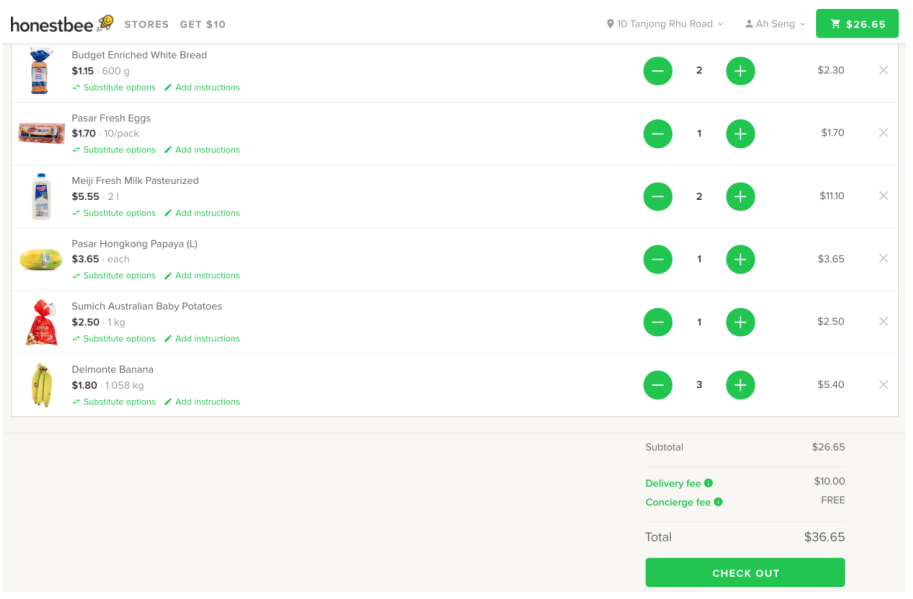
\includegraphics[width=0.6\paperwidth]{C:/Users/Admin/Desktop/Github/question_bank/LyX/static/img/9597-DHS-2016-P2-Q6-1}
\par\end{center}

In the event that the item is out of stock, the customer can also
opt for 3 options: 
\begin{center}
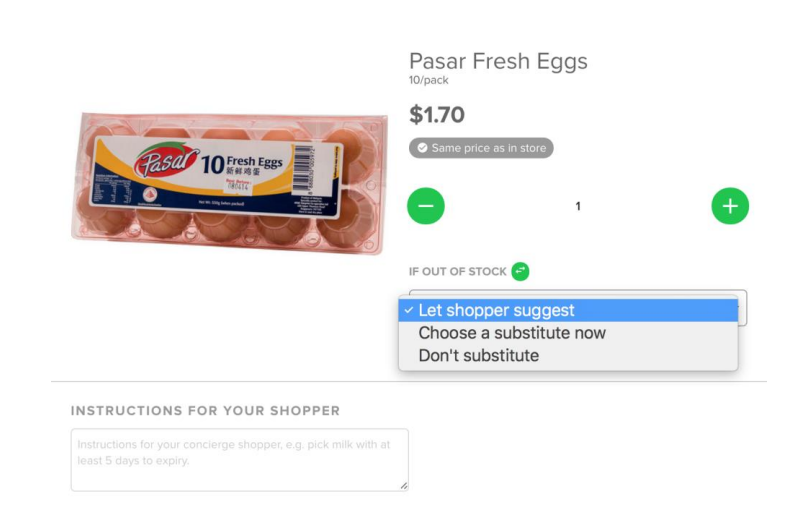
\includegraphics[width=0.6\paperwidth]{C:/Users/Admin/Desktop/Github/question_bank/LyX/static/img/9597-DHS-2016-P2-Q6-2}
\par\end{center}
\begin{enumerate}
\item Produce a normalised relational database schema showing the table
specifications. \hfill{}{[}8{]}
\item Draw an ER diagram illustrating the entities and their relationships.
\hfill{}{[}3{]}
\item Using suitable examples from this context, explain the concepts of
\begin{enumerate}
\item primary key (for the Customer table) \hfill{}{[}2{]}
\item composite key \hfill{}{[}2{]}
\item foreign key \hfill{}{[}2{]}
\end{enumerate}
\item Orders below \$30 is charged a delivery fee of \$10, else delivery
fee is waived. Some orders may incur a concierge fee for special instructions.
Where should fields such as delivery fee and concierge fee be stored?
Why? \hfill{}{[}2{]}
\end{enumerate}